\begin{mainquestion}{nodaldependentsource}{Dependent Source Circuit}

\questionpoints Calculate $v_x$ in the circuit below using nodal analysis.

\begin{center}
    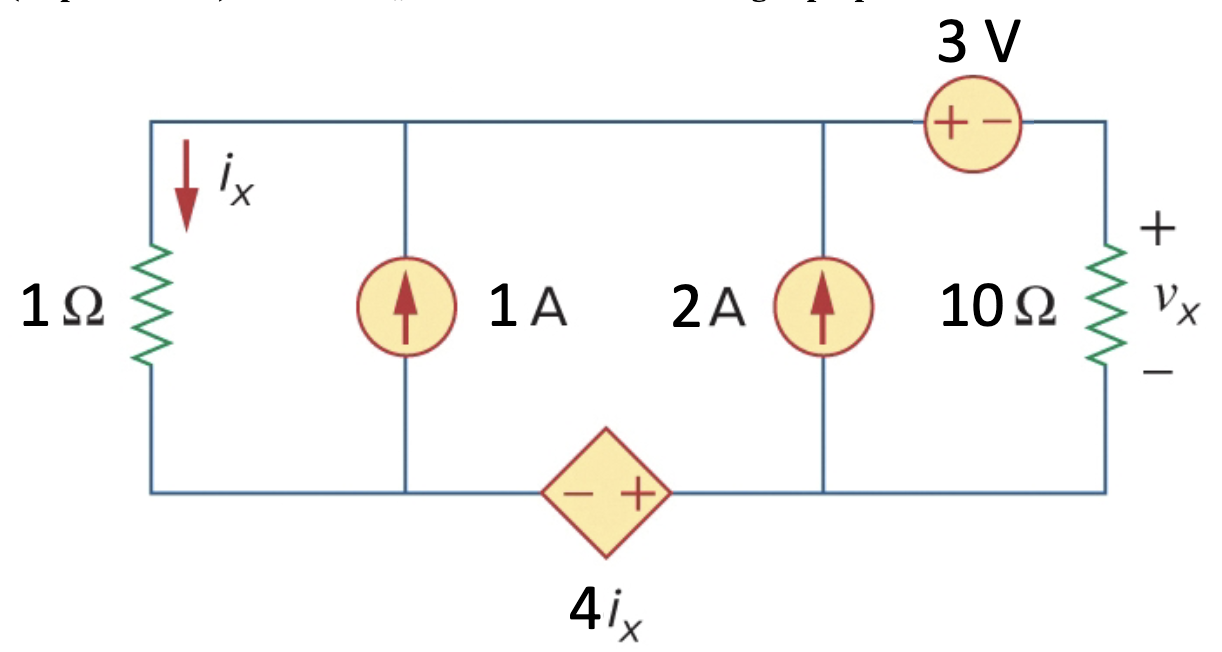
\includegraphics[width=0.6\textwidth]{dependentsources.png}
\end{center}

\begin{answer}
\textbf{Step 1: Define node voltages}

Let the bottom-left node be the reference node (ground).
Let the top-left node voltage be $V_1$ and the top-right node voltage be $V_2$.

The current $i_x$ flows downward through the $1\,\Omega$ resistor, so:
\[
i_x = \frac{V_1 - 0}{1} = V_1.
\]

\medskip
\textbf{Step 2: Apply voltage constraints}

The $3\,\text{V}$ source on the top rail enforces:
\[
V_1 - V_2 = 3
\quad \Rightarrow \quad
V_2 = V_1 - 3.
\tag{1}
\]

The dependent voltage source on the bottom rail has value $4i_x$ with polarity
from left to right, so the bottom-right node voltage is:
\[
V_{\text{bottom-right}} = 4i_x = 4V_1.
\tag{2}
\]

\medskip
\textbf{Step 3: Write KCL at the supernode}

The supernode consists of the two top nodes connected by the $3\,\text{V}$ source.

Currents entering the supernode:
\[
1\,\text{A} + 2\,\text{A} = 3\,\text{A}.
\]

Currents leaving the supernode:
\[
\text{through } 1\,\Omega: \quad V_1,
\]
\[
\text{through } 10\,\Omega: \quad \frac{V_2 - V_{\text{bottom-right}}}{10}
= \frac{V_2 - 4V_1}{10}.
\]

Applying KCL:
\[
3 = V_1 + \frac{V_2 - 4V_1}{10}.
\tag{3}
\]

\medskip
\textbf{Step 4: Solve}

Substitute Eq.~(1) into Eq.~(3):
\[
3 = V_1 + \frac{(V_1 - 3) - 4V_1}{10}.
\]

\[
3 = V_1 + \frac{-3V_1 - 3}{10}.
\]

\[
30 = 10V_1 - 3V_1 - 3.
\]

\[
7V_1 = 33
\quad \Rightarrow \quad
V_1 = \frac{33}{7}.
\]

\medskip
\textbf{Step 5: Compute $v_x$}

The voltage across the $10\,\Omega$ resistor is:
\[
v_x = V_2 - V_{\text{bottom-right}}.
\]

Using Eqs.~(1) and (2):
\[
V_2 = \frac{33}{7} - 3 = \frac{12}{7},
\quad
V_{\text{bottom-right}} = \frac{132}{7}.
\]

\[
v_x = \frac{12}{7} - \frac{132}{7}
= \boxed{-\frac{120}{7}\,\text{V}}.
\]

\[
\boxed{v_x \approx -17.1\,\text{V}}
\]
\end{answer}

\end{mainquestion}
